%%%%%%%%%%%%%%%%%%%%%%%%%%%%%%%%%%%%%%%%%%%
%   Simple and elegant academic report    %
%   Copyright by Artur M. Brodzki, 2019   %
%%%%%%%%%%%%%%%%%%%%%%%%%%%%%%%%%%%%%%%%%%%

\documentclass{eiti-raport}

\usepackage[
	english,
	polish
]{babel}
\usepackage{polski}
\usepackage{listings}

%------------------------------------------

\begin{document}

\author{Artur M. Brodzki \\ Damian Chiliński \\ Krzysztof Sznejder}
\date{\today}
\subject{BCYB 19L}
\title{Projekt -- dokumentacja koŃcowa}
\fancyhead[L]{Brodzki, Chiliński, Sznejder}
\fancyhead[R]{BCYB 19L}

\pagenumbering{arabic}
\maketitle

%------------------------------------------
% MAIN CONTENTS
%------------------------------------------

\section{Wstęp} \label{sec:intro}
Zgodnie z przyjętym przez nas tematem, w ramach projektu napisaliśmy moduł systemu IDS/IPS Snort, wykrywający steganograficzną transmisję danych metodą tunelowania DNS. Przetestowaliśmy również jego działanie w wirtualnym środowisku, symulującym sieć korporacyjną. 

\section{Tunelowanie DNS} \label{sec:2}

\subsection{Zasada działania} \label{sec:tunelowanie}
Tunelowanie DNS należy do metod steganograficznych i pozwala na prowadzenie niewidocznej dla administratorów transmisji danych, np. przesłanie na maszynę atakującego wykradzionych plików. Zasada działania opiera się na redundancji protokołu DNS. Typowy przebieg ataku z wykorzystaniem tunelowania DNS jest następujący:
\begin{enumerate}
	\item Atakujący rejestruje domenę, np. \texttt{best-malware.com} i tworzy dla niej własny serwer autorytatywny. 
	\item Atakujący instaluje złośliwe oprogramowanie na systemach ofiary, które wykrada z nich wrażliwe dane, np. hasło bankowe. 
	\item Oprogramowanie atakującego koduje uzyskane informacje jako subdomenę, np: \\  \texttt{76756C6E657261626C65.bestmalware.win} i wysyła odpowiadające jej zapytanie DNS. Trafia ono na serwer atakującego, który może odebrać i zdekodować ukryte informacje. Dane można kodować zasadniczo za pomocą kodowania szesnastkowego lub base32. Wynika to ze specyfikacji protokołu DNS, który dopuszcza w zapytaniach ograniczony zestaw znaków. 
	\item Aby przeprowadzić transmisję w drugą stronę, wystarczy zakodować informację w pakiecie będącym odpowiedzią na zapytanie. Najczęściej będzie to więc pakiet typu A, choć możliwe jest kodowanie danych z użyciem każdego typu rekodu DNS. 
\end{enumerate}
Skuteczność tego ataku wynika z kluczowej roli, jaką odgrywa DNS w komunikacji internetowej. Jego zablokowanie może uniemożliwić działanie sieci, dlatego zapytania DNS bardzo rzadko są ograniczane przez administratorów, i to nawet w sieciach o restrykcyjnych wymogach bezpieczeństwa. 

\subsection{Metody wykrywania} \label{sec:wykrywanie}
Aby skutecznie zablokować transmisję wykorzystującą tunelowanie DNS, konieczne jest wiarygodne odróżnienie złośliwych zapytań DNS od tych prawidłowych. Stosuje się w tym celu zbiór heurystyk, opartych m.in. o:
\begin{itemize}
	\item analizę długości i entropii zapytania -- większość ,,normalnych'' domen nie przekracza kilkunastu znaków i charakteryzuje się niewielką entropią, typową dla słów pochodzących z języka naturalnego;
	\item analizę częstości -- znaczący wzrost liczby wykonywanych zapytań DNS może sugerować, że część z nich jest niepożądana;
	\item metody słownikowe -- ,,prawdziwe'' domeny zazwyczaj składają się ze słów pochodzących z języka naturalnego lub zbudowanych na ich podstawie neologizmów;
	\item uczenie maszynowe.
\end{itemize}
W naszym projekcie zdecydowaliśmy się wykorzystać autorski algorytm uczenia maszynowego oparty o naiwny klasyfikator Bayesa. Klasyfikator został nauczony na zbiorze zapytań DNS wygenerowanych i przechwyconych przez nas podczas kilku tygodni codziennego użytkowania naszych domowych komputerów. Szczegółowy opis algorytmu znajduje się w sekcji \ref{sec:plugin} 

\section{Scenariusz projektowy} \label{sec:scenariusz}
Zaplanowaliśmy następujący scenariusz projektowy: firma B-Cyb S.A dysponuje siecią korporacyjną, działającą w domenie \texttt{bcyb.com}. W ramach świadczonych usług, posiada dwa publicznie dostępne serwery HTTP, kolejno: \texttt{s1.bcyb.com} oraz \texttt{s1.bcyb.com}. Dostęp do firmowej sieci chroniony jest za pomocą firewalla działającego na firmowym routerze, jak również z użyciem systemu IDS/IPS Snort, filtrującego ruch przepływający przez sieć. Ponieważ firma B-Cyb obawia się ataku metodą tunelowania DNS, zakupiła od młodego zespołu specjalistów (Kant Security sp. z.o.o) dodatkowy moduł systemu Snort, mający wykrywać i blokować tego rodzaju ataki. W ramach sieci firmowej została wydzielona podsieć, chroniona -- w celach testowych -- przy użyciu nowego modułu. 

Na firmowych serwerach znajduje się jednak złośliwe oprogramowanie, którego zadaniem jest przetransmitować na serwery atakującego wykradzione pliki \texttt{/etc/shadow}. Ponieważ wyprowadzenie danych poza sieć za pomocą protokołu TCP jest niemożliwe, atakujący zdecydowali się zastosować właśnie tunelowanie DNS. Podczas próby przesłania wykradzionych haseł, nowy moduł Snorta od zespołu Kant Security wykryje i zablokuje złośliwą transmisję. Natomiast podsieć chroniona za pomocą dotychczasowej wersji systemu Snort nie wykryje ataku i pozwoli na wyprowadzenie haseł na zewnątrz. 

Całość infrastruktury projektowej została zainstalowana przez nas na maszynach wirtualnych VMware i obejmuje łącznie 9 hostów, znajdujących się pod kontrolą systemu Fedora 30. Szczegółowa topologia sieci znajduje się na rys. \ref{fig:topologia}. 
\begin{figure}[!h] \centering
	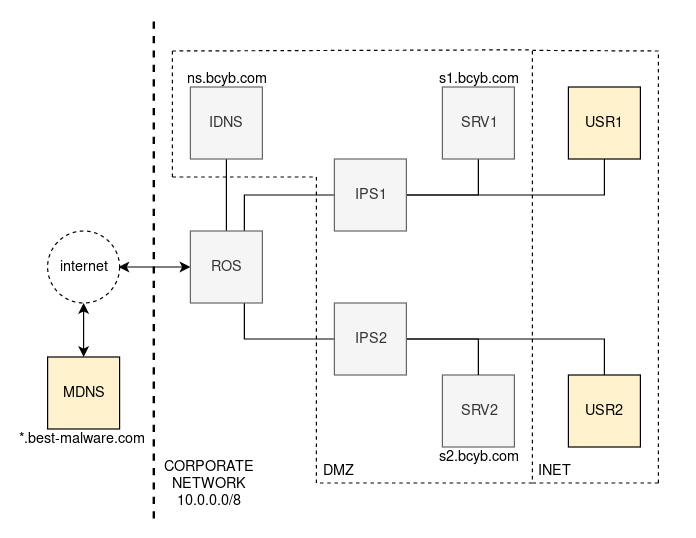
\includegraphics[width=0.9\linewidth]{img/BCYB_topologia.png}
	\caption{Schemat ideowy sieci, realizującej przyjęty scenariusz projektowy.} \label{fig:topologia}
\end{figure}
Przygotowana infrastruktura składa się z następujących urządzeń: 
\begin{itemize}
	\item router ROS: domyślna brama sieciowa dla sieci firmowej, działa pod kontrolą systemu MikroTik RouterOS i obsługuje zaporę sieciową;
	\item IDNS: firmowy serwer DNS;
	\item SRV1 i SRV2: publicznie dostępne serwery HTTP;
	\item IPS1 i IPS2: hosty systemu Snort, działające w trybie inline i filtrujące ruch przechodzący przez sieć;
	\item USR1 i USR2: komputery użytkowe, służące pracownikom firmy do wykonywania obowiązków służbowych, w tym zarządzania pozostałymi hostami;
	\item MDNS: komputer atakującego, stanowiący punkt odbiorczy ukrytej komunikacji. 
\end{itemize}
Zapora sieciowa posiada następującą konfigurację:
\begin{enumerate}
	\item sieć firmowa (corporate network, 10.0.0.0/8) podzielona jest na strefę zdemilitaryzowaną (DMZ) oraz sieć wewnętrzną (INET);
	\item strefa zdemilitaryzowana: obejmuje publicznie dostępne serwery DNS i HTTP (IDNS, SRV1, SRV2), jak również chroniące je hosty systemu Snort.
	\begin{itemize}
		\item ruch wchodzący: dopuszczony jest jedynie ruch realizujący świadczone usługi, oraz ruch SSH pochodzący z sieci INET;
		\item ruch wychodzący: zabronione jest inicjowanie ruchu w obrębie DMZ, z wyjątkiem zapytań DNS oraz ruchu wychodzącego do serwerów zawierających repozytoria Fedory. Dopuszczony jest zatem jedynie ruch wymagany do pobierania aktualizacji oprogramowania systemowego;
	\end{itemize}
	\item sieć wewnętrzna: obejmuje komputery służbowe USR1 i USR2:
	\begin{itemize}
		\item ruch wchodzący: jest zasadniczo zabroniony w każdym przypadku i na wszystkich portach, dopuszczony jest jednak rzecz jasna ruch powrotny w ramach połączeń zainicjowanych przez hosty sieci INET (connection-state=establieshed,related).
		\item ruch wychodzący: co do zasady nie jest filtrowany, z wyjątkiem ograniczeń wymuszonych przez zaporę dla ruchu wchodzącego do DMZ.
	\end{itemize}
\end{enumerate}
Z uwagi na nietrywialną złożoność wirtualizowanej infrastruktury, istotne jest określenie wymagań sprzętowych. Szczególnie ważna jest ilość pamięci operacyjnej, wymagana do działania poszczególnych hostów:
\begin{itemize}
	\item każdy z hostów posiadających graficzny interfejs użytkownika (USR1, USR2, MDNS) wymaga 2 GB pamięci RAM;
	\item hosty systemu Snort (IPS1, IPS2) wymagają do sprawnego działa po 768 MB pamięci RAM każdy;
	\item serwery HTTP (SRV1, SRV2) zajmują po 512 MB pamięci;
	\item do działania serwera DNS (IDNS) konieczne jest 512 MB, a dla routera ROS -- 256 MB pamięci RAM.
\end{itemize}
Doliczając do tego pamięć systemu gospodarza okazuje się, że dla uruchomienia całej wymaganej infrastruktury niezbędne jest co najmniej 12 GB pamięci operacyjnej. W praktyce będzie to zazwyczaj 16 GB. 

Istotnym zagadnieniem był również wybór wersji systemu Snort. Aktualna wersja stabilna to 2.9.13, jednak prace deweloperskie koncentrują się na Snorcie 3, który wciąż znajduje się w wersji beta, a data jego finalnego wydania pozostaje nieznana. Snort 3 jest zupełnie nowym programem napisanym od zera i niekompatybilnym wstecznie ze Snortem 2. Z punktu widzenia naszego projektu charakteryzuje się jednak ważną zaletą: jego API zostało zaprojektowane z myślą o tworzeniu wtyczek rozszerzających funkcjonalność systemu. Pomimo znacznych braków w dokumentacji zdecydowaliśmy się zatem na przygotowanie naszej wtyczki dla Snorta 3. 

\section{Implementacja} \label{sec:implementation}

\subsection{Aplikacja nadawcza i odbiorcza} \label{sec:dnsenc}
Aplikacje nadawcza i odbiorcza, realizujące transmisję metodą tunelowania DNS, znajdują się w repozytorium projektu w katalogu \texttt{./dns\_tools}:
\begin{itemize}
	\item skrypt \texttt{dnsenc.sh} stanowi aplikację nadawczą i przyjmuje dwa argumenty, kolejno: plik do wysłania i domenę docelową. Jego działanie polega na zakodowaniu wysyłanego pliku w formacie base32 i podzieleniu go na 8-znakowe fragmenty. Każdy fragment wysyłany jest jako subdomena zapytania DNS, jak opisano w rozdziale \ref{sec:tunelowanie}. Zapytania DNS generowane są za pomocą dostępnego w systemie Linux narzędzia \texttt{nslookup}. 
	\item skrypt \texttt{dnsdec.js} jest napisany jako skrypt NodeJS i stanowi aplikację odbiorczą. Przyjmuje jeden argument: domenę, dla której nasłuchujemy przychodzących zapytań. Zdekodowane dane wypisywane są domyślnie na standardowe wejście, skąd mogą zostać przekierowane do pliku. 
\end{itemize}

\subsection{Podstawowy algorytm klasyfikacji} \label{sec:bayes}
Algorytm klasyfikacji zapytań DNS wykorzystuje naiwny klasyfikator Bayesa na engramach. Działanie klasyfikatora opiera się na obserwacji, że pewne sekwencje znaków (engramy) występują znacznie częściej w naturalnych domenach DNS niż w zakodowanych danych binarnych, a inne -- odwrotnie. Zdecydowaliśmy się wykorzystać engramy długości 3, jako kompromis pomiędzy dokładnością klasyfikatora a wymaganą złożonością obliczeniową. W naszym zbiorze występują subdomeny używające łącznie 38 znaków, możliwe są więc 54 872 różne trójznaki, z czego 37 425 istotnie wystąpiło przynajmniej raz w zbiorze uczącym. 

Częstości najczęściej występujących trójznaków dla obu przypadków przedstawione są (w skali logarytmicznej) na rys. \ref{fig:engrams-hist}. Widoczne jest, że o ile w przypadku danych binarnych wszystkie trójznaki występują z niemal identyczną częstością (duża entropia rozkładu), to dla ,,naturalnych'' domen DNS zachodzi znaczna koncentracja: istnieje pewien niewielki zbiór trójznaków o znacznej częstości i wiele innych występujących bardzo rzadko (mała entropia rozkładu). 
\begin{figure}[!h] \centering
	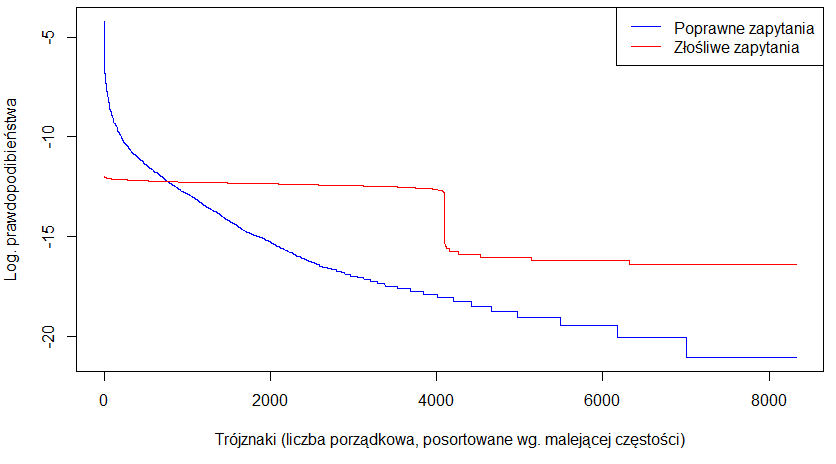
\includegraphics[width=0.9\linewidth]{img/engrams-hist.PNG}
	\caption{Częstości występowania najczęstszych trójznaków w obu klasach zapytań.} \label{fig:engrams-hist}
\end{figure}
Widoczny dla danych binarnych ,,uskok'' w połowie wykresu wynika z obecności w zbiorze uczącym dwóch metod kodowania, tj. hex i base32. Ponieważ zbiór znaków szesnastkowych niemal w całości zawiera się w zbiorze znaków dopuszczalnych dla kodowania base32, to pewne trójznaki możliwe są w obu metodach kodowania (np. 456, AAA), natomiast inne -- możliwe są tylko w kodowaniu base32 (np. ZZZ). Te drugie są odpowiednio rzadsze. 

Klasyfikator może popełnić dwa rodzaje błędów: \emph{false-positive} i \emph{false-negative}. Należy zauważyć, że w naszym przypadku koszt błędu typu \emph{false-negative} jest znacznie większy, niż \emph{false-positive}. W przypadku przepuszczenia kilku złośliwych zapytań grozi nam co najwyżej przesłanie niewielkiej ilości wykradzionych danych, rzędu kilka-kilkanaście bajtów, natomiast w przypadku zablokowania zapytań poprawnych grozi nam utrata funkcjonalności sieci. Z tego względu istotne jest maksymalne zwiększenie czułości klasyfikatora, nawet kosztem jego mniejszej precyzji (ang. \emph{precision and recall}). 

Podstawowym parametrem wpływającym na jakość klasyfikacji zadanej subdomeny jest jej długość: dłuższe domeny znacznie łatwiej jest poprawnie sklasyfikować, ze względu na większą ilość dostępnej informacji. W skrajnym przypadku domeny jednoznakowej np. \texttt{a.best-malware.com} niemożliwe jest stwierdzenie, czy jest ona poprawna, czy też stanowi 4 bity danych binarnych zakodowanych szesnastkowo, lub 5 bitów danych w formacie base32. Ze względu na wykorzystanie przez nas trójznaków, minimalna długość subdomeny, jaką nasz klasyfikator jest w stanie sklasyfikować, wynosi 3. Można rozważać podniesienie tego limitu, w celu uniknięcia błędów typu \emph{false-negative} i zwiększenia czułości. Rys. \ref{fig:length-hist} przedstawia histogram częstości subdomen w zależności od ich długości. 
\begin{figure}[!h] \centering
	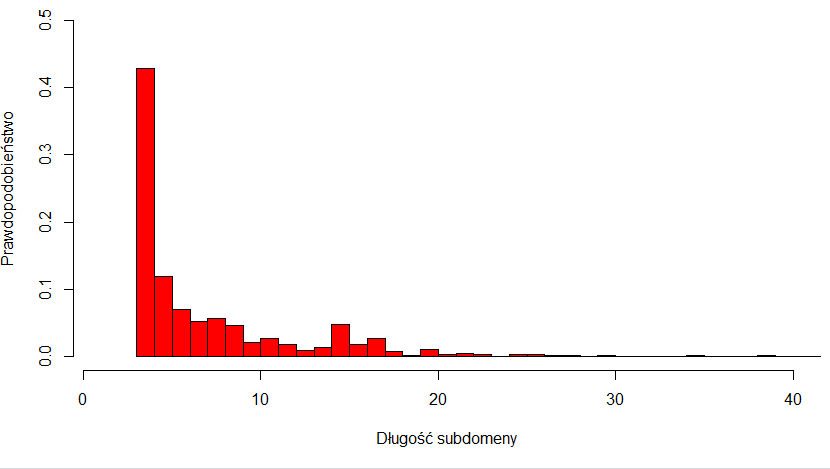
\includegraphics[width=0.9\linewidth]{img/length-hist.PNG}
	\caption{Histogram długości subdomen w ,,naturalnych'' zapytaniach DNS.} \label{fig:length-hist}
\end{figure}
Widoczna jest wyraźna dominanta rozkładu dla 3 znaków, co wynika z tego, że zdecydowanie najczęstszą subdomeną jest \texttt{www}, oraz częste występowanie stosunkowo krótkich domen (< 5 znaków). Z tego względu ich klasyfikacja jest łatwa i ostatecznie zdecydowaliśmy, że nasz klasyfikator będzie klasyfikował domeny o minimalnej długości 3 znaków. Uzyskana czułość okazała się wystarczająca. Krótsze subdomeny nie podlegają klasyfikacji, a zatem są one zawsze przepuszczane. 

Algorytm klasyfikacji pojedynczej subdomeny przedstawia się następująco. Dla zadanej domeny, kolejne trójznaki generowane są metodą okna przesuwnego, np. domenie
\begin{align*}
d = \texttt{tunelowanie.bcyb.com}
\end{align*}
odpowiada wektor trójznaków 
\begin{align*}
\vec{3}(d) = \left[ \texttt{tun}, \texttt{une}, \texttt{nel}, \texttt{elo}, \texttt{low}, \texttt{owa}, \texttt{wan}, \texttt{ani}, \texttt{nie} \right]
\end{align*}
W fazie trenowania obliczana jest względna częstość występowania poszczególnych trójznaków $s$ na całym zbiorze uczącym, w klasie pozytywnej $P$ (zapytania poprawne) i negatywnej $N$ (zapytania złośliwe), według następującego wzoru:
\begin{align*}
v(s) = \log_2 \left( \frac{p\left(s|P\right)}{p\left(s|N\right)} \right) = \log_2 p\left(s|P\right) - \log_2 p\left(s|N\right) 
\end{align*}
Wartość $v(s)$ jest dodatnia, gdy $p(s|P) > p(s|N)$ oraz ujemna, gdy $p(s|N) > p(s|P)$. W przypadku, gdy $p(s|P) = 0$ ($s$ występuje tylko w klasie negatywnej), przyjmuje się $v(s) = -100$. Jeśli $p(s|N) = 0$ ($s$ występuje tylko w klasie pozytywnej) przyjmuje się $v(s) = 100$. W praktyce, zdecydowana większość trójznaków występuje tylko w jednej klasie, co pozwala na szybkie i jednoznaczne sklasyfikowanie większości zapytań. 

Skrypt \texttt{./ips\_dns\_tunnel/bayes/train.r} generuje plik CSV, zawierający uszeregowany alfabetycznie zbiór wszystkich trójznaków wraz z odpowiadającymi im wartościami $v(s)$. Plik ten jest wczytywany przez Snorta, a następnie wykorzystywany do klasyfikacji zapytań. Dla subdomeny $d$ wyznacza się jej klasę $C(d)$, według następującego wzoru:
\begin{align*}
\text{val}(d) & = \sum_{s \in \vec{3}(d)} v(s) \\ \\ 
C(d) & = \begin{cases}
	P & \text{for} \ \text{val}(d) > \textrm{thr} \\ 
	N & \text{w.p.p.}
\end{cases}
\end{align*}
gdzie $\textrm{thr}$ stanowi przyjęty próg klasyfikacji. Wartość tego progu wprost wpływa na czułość klasyfikatora, która rośnie wraz ze zmniejszaniem progu. Dla $\text{thr} = 0$ mamy proste porównanie prawdopodobieństw: wybierana jest klasa o większym szacowanym prawdopodobieństwie. Dla $\text{thr} < 0$ prawdopodobieństwo klasy negatywnej powinno być odpowiednio większe, dla zaklasyfikowania subdomeny jako złośliwej. Metodą prób i błędów, przyjęliśmy $\text{thr} = \log_2 20 \approx 4,32$, co stanowi kompromis pomiędzy brakiem fałszywych alarmów a dość szybkim blokowaniem złośliwej transmisji. 

Uzyskane wartości czułości i precyzji różnią się diametralnie pomiędzy witrynami, nie będziemy więc tutaj przytaczać konkretnych liczb; oscylują one zazwyczaj pomiędzy 0,96-0,99 dla czułości i 0,8-0,95 dla precyzji. Oznacza to, że o ile zapytania złośliwe są wykrywane bardzo skutecznie (mamy 80-90\% szans na zablokowanie złośliwej transmisji już po jednym zapytaniu), to średnio kilka procent zapytań poprawnych klasyfikowanych jest jako złośliwe. Rodzi to znaczne ryzyko niestabilnego działania sieci końcowego użytkownika. Niestety, próby zmniejszenia tego wyniku poprzez ulepszenie klasyfikatora, są w zasadzie skazane na niepowodzenie, niezależnie od użytej metody uczenia maszynowego. Okazuje się bowiem, że w również w ,,naturalnych'' zapytaniach DNS zdarza się deweloperom umieszczać dane binarne, np. kodowane szesnastkowo sumy kontrolne MD5. Przykłady takiej praktyki przedstawiono na rys. \ref{fig:badlog}. 
\begin{figure}[!h] \centering
	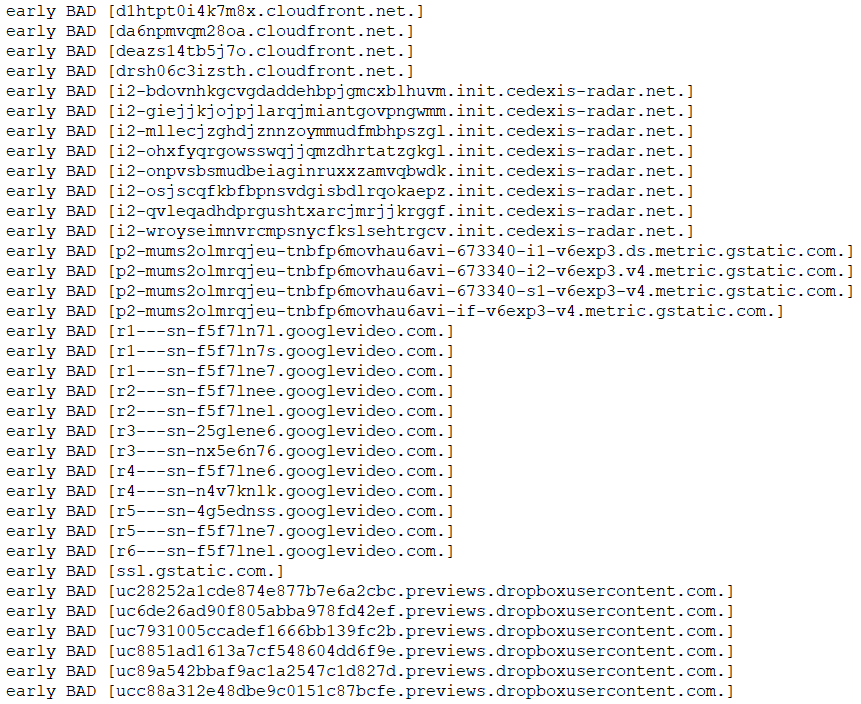
\includegraphics[width=0.95\linewidth]{img/badlog.PNG}
	\caption{Przykłady ,,naturalnych'' zapytań DNS zawierających kodowane dane binarne.} \label{fig:badlog}
\end{figure}

Z tego względu, niemożliwe jest odrzucanie zapytań do zadanej domeny tylko i wyłącznie na podstawie klasyfikatora Bayesa -- bardzo szybko doprowadziłoby to do uniemożliwienia działania większości witryn. Ostateczny klasyfikator stosuje zatem rozszerzoną analizę częstotliwościową. Została ona opisana w szczegółach w następnym podrozdziale. 

\subsection{Wtyczka systemu Snort} \label{sec:plugin}

Narzędzia służące do wykrywania tunelowania DNS znajdują się w katalogu \texttt{./ips\_dns\_tunnel}. Obok znajdujących się w podkatalogu \texttt{bayes} i opisanych już wyżej skryptów R, mamy kolejno podkatalogi:
\begin{itemize}
	\item \texttt{snort\_plugin}: kod właściwej wtyczki w języku C++, kompilowany (podobnie jak cały Snort) za pomocą CMake;
	\item \texttt{snortd}: daemon systemd (ang. \emph{systemd unit}), uruchamiający Snorta automatycznie podczas startu systemu. Działa on na hostach IPS1/IPS2 i umożliwia ich działanie w trybie inline bez dodatkowej ingerencji ze strony użytkownika. 
\end{itemize} 
Jak wskazano w rozdziale \ref{sec:bayes}, ,,surowy'' klasyfikator Bayesa wymaga dalszych usprawnień. Ostateczny algorytm klasyfikacji realizowany przez naszą wtyczkę działa następująco:
\begin{enumerate}
	\item Dla każdej odpytywanej domeny pierwszego poziomu (np. \texttt{google.com}, \texttt{cloudflare.com}) tworzona jest tablica $T$ o długości $N$;
	\item wpisy w tablicy zawierają $N$ ostatnich \emph{unikalnych} subdomen, odpytywanych w ramach tej domeny; wielokrotne zapytania kierowane do tej samej subdomeny, np. \texttt{www.cloudflare.com} stanowią jeden wpis;
	\item dla każdej subdomeny tabela przechowuje informację, do jakiej klasy została ona przypisana przez surowy klasyfikator Bayesa;
	\item w momencie, gdy łączna długość subdomen znajdujących się w danej tablicy i zaklasyfikowanych jako złośliwe przekroczy zadany próg $L$ znaków, cała domena pierwszego poziomu jest blokowana, a wszystkie kierowane do niej zapytania są odrzucane.
\end{enumerate}
Skuteczność tego algorytmu bierze się w faktu, że proces pojawiania się wpisów w tabeli $T$ można modelować (w przybliżeniu) jako proces Poissona. Przy założeniu, że prawdopodobieństwo zdarzenia typu \emph{false-negative} jest stałe i niezależne od historii zapytań\footnote{Jest to założenie w praktyce niespełnione, ale zachodzi ono w stopniu wystarczającym do działania algorytmu.}, ryzyko zablokowania zaufanej domeny daje się opisać za pomocą rozkładu Poissona.

Załóżmy, że średnia długość subdomeny w zapytaniu wynosi $z$ znaków, a prawdopodobieństwo zajścia zdarzenia typu \emph{false-negative} wynosi $p$. Liczba domen w tablicy jest równa $N$, z czego średnio $pN$ będzie zakwalifikowane jako złośliwe. Liczba $pN$ odpowiada zatem parametrowi $\lambda$ rozkładu Poissona $f(k,\lambda)$, a prawdopodobieństwo wystąpienia w tabeli dokładnie $k$ domen zakwalifikowanych jako złośliwe wynosi 
\begin{align}
f(k,pN) = \left( e^{-pN} \right) \frac{ \left( pN \right)^k }{k!}
\end{align}
Do zablokowania domeny wymagane jest co najmniej $\frac{L}{z}$ zablokowanych subdomen, zatem prawdopodobieństwo błędnego zablokowania domeny wynosi:
\begin{align} \label{eq:cumulative}
P\left( k > Lz^{-1} \right) = e^{-pN} \sum_{k = Lz^{-1}}^{N} \frac{ \left( pN \right)^k }{k!}
\end{align}
Jak wprost wynika ze wzoru \ref{eq:cumulative}, ryzyko fałszywego alarmu maleje wykładniczo wraz ze wzrostem długości tablicy $T$, jednocześnie jednak jej zwiększanie powoduje wzrost ilości pamięci wymaganej do działania wtyczki; należy pamiętać, że w ciągu jednego dnia użytkowania komputer osobisty jest on w stanie odpytać od kilkuset do kilku tysięcy różnych domen pierwszego poziomu. Wartości $N$ i $L$ stanowią parametry uruchomieniowe przygotowanej przez nas wtyczki i wprost decydują o jej skuteczności w codziennym użytkowaniu. Metodą prób i błedów, za optymalną przyjęliśmy konfigurację ,,32/72'', czyli tablicę długość tablicy $T$: $N = 32$ wpisy i próg blokady $L = 72$ znaki. Dla takich wartości $N$ i $L$, średniej długości zapytania równej $z = 8$ znaków oraz współczynniku \emph{false-negative} $p = 2\%$, teoretyczne prawdopodobieństwo uzyskania fałszywego alarmu wynosi:
\begin{align*}
P \left( k > 9 \right) = 2.8 \cdot 10^{-8}
\end{align*}
czyli $0.0000028\%$ na zapytanie. Dla średniej ilości zapytań rzędu kilka tysięcy dziennie, daje to teoretycznie jeden fałszywy alarm na 10,000 dni użytkowania. 

\section{Testy}
Jak wspomniano, w rzeczywistości założenia procesu Poissona są niespełnione i prawdopodobieństwo fałszywego alarmu jest o 3-4 rzędy wielkości większe od wartości teoretycznej. Na dodatek, jest ono silnie zależne od konkretnej witryny. Niektóre strony, jak np. Cloudflare, generują bardzo duże ilości subdomen o charakterze danych binarnych i są szybko blokowane, niezależnie od długości tablicy i pozostałych parametrów klasyfikatora. Z tego względu, nasza wtyczka posiada również funkcję białej listy: listy zaufanych domen, które nie podlegają blokowaniu. Użytkownik końcowy ma możliwość dostosowania działania wtyczki do swoich własnych potrzeb. 

Oprócz prawidłowej klasyfikacji zaufanych zapytań DNS, zadaniem wtyczki jest również blokować zapytania niepożądanych. Skuteczność wtyczki w tym zakresie jest znaczna; jak przedstawiono na rys. \ref{fig:engrams-hist}, statystyka engramów dla zapytań złośliwych różni się znacznie od ,,nauralnych'' i ich odróżnienie nie stanowi trudności. Z uwagi na przyjęty próg blokady domeny $L = 72$ znaki oraz precyzję klasyfikatora rzędu 0.8-0.9, zablokowanie złośliwej transmisji następuje już po kilku-kilkunastu zapytaniach. Pozwala to na przesłanie co najwyżej kilkudziesięciu bajtów danych. Odpowiednia demostracja działania zostanie przedstawiona podczas prezentacji na koniec semestru. 

\section{Podsumowanie} \label{sec:summary}
Celem projektu było przygotowanie wtyczki dla systemu IDS/IPS Snort, służącej do blokowania ukrytej transmisji metodą tunelowania DNS. Uzyskane wyniki uznajemy za zadowalające, zarówno pod względem przepuszczania prawidłowych zapytań jak i blokowania zapytań złośliwych. Projekt był szczególnie rozwijający z uwagi na konieczność skonfigurowania nietrywialnej sieci korporacyjnej oraz zestawu jej zabezpieczeń: zapory ogniowej oraz systemu IDS/IPS Snort 3. 

\end{document}
